\documentclass[10pt,a4paper]{article}
\usepackage[margin=0.82in,headheight=14pt]{geometry}
\usepackage[T1]{fontenc}
\usepackage{lmodern,microtype}
\usepackage{amsmath,amssymb}
\usepackage{booktabs,tabularx,array}
\usepackage{graphicx}
\usepackage{xcolor}
\usepackage{tikz}
\usepackage{siunitx}
\usepackage{hyperref}
\usepackage{fancyhdr}
\usepackage{caption}
\usepackage{placeins}
\usetikzlibrary{arrows.meta,decorations.pathmorphing}

\definecolor{ink}{HTML}{18313F}
\definecolor{accent}{HTML}{00677A}
\definecolor{warm}{HTML}{B44A25}
\definecolor{muted}{HTML}{52636A}
\hypersetup{colorlinks=true,linkcolor=accent,citecolor=accent,urlcolor=accent}
\sisetup{detect-all,per-mode=symbol}
\captionsetup{font=small,labelfont=bf}
\setlength{\parindent}{0pt}
\setlength{\parskip}{0.42em}
\setlength{\textfloatsep}{12pt plus 3pt minus 2pt}
\pagestyle{fancy}
\fancyhf{}
\fancyhead[L]{\small\textcolor{muted}{Advanced Control Theory}}
\fancyhead[R]{\small\textcolor{muted}{Quarter-car AFC reproduction}}
\fancyfoot[C]{\thepage}

\title{\textbf{Approximation-Free Active Suspension Control}\large\\[0.25em]
Paper analysis and a MATLAB/Simulink quarter-car reproduction}
\author{Advanced Control Theory course project}
\date{30 September 2026}

\begin{document}
\maketitle
\vspace{-1.5em}

\begin{abstract}
Na et al. proposed an approximation-free control (AFC) law with prescribed performance functions (PPFs) for an electro-hydraulic quarter-car suspension and experimentally evaluated it against backstepping and PID control. This report reconstructs the paper's control logic, implements a five-state sampled-data MATLAB model and an editable Simulink counterpart, and audits the resulting trajectories with independently generated figures. The available publication does not provide the full identified rig/valve constants or raw time histories, so the present simulation uses explicitly documented representative values. For a \SI{0.043}{m}, \SI{0.505}{Hz} sinusoidal road input, the simulated AFC reduces displacement IAE relative to passive suspension (0.4849 versus 0.6709\,m\,s), but it reaches the \(\pm\SI{5}{V}\) rail for 85.4\% of samples and violates the nominal displacement envelope by up to \SI{0.01885}{m}. These findings are a reproducibility and actuator-feasibility diagnostic, not a numerical refutation or a hardware replication of the original paper.
\end{abstract}

\noindent\textbf{Evidence convention.} \textsc{Paper} denotes results reported by Na et al.; \textsc{Simulation} denotes this project's outputs; \textsc{Assumption} denotes a parameter not identified for the target rig.

\section{Research question and source paper}
Ride comfort calls for low sprung-mass displacement and acceleration under road excitation, while the hydraulic valve must obey finite voltage and pressure constraints. The source paper asks whether a lightweight recursive controller can enforce a prescribed displacement transient without online function approximation, and whether that design remains practical on a physical electro-hydraulic quarter-car rig \cite{na2022}. Its contribution is the combination of a transformed-error AFC design, a prescribed-performance envelope, and experimental comparison with backstepping control (BSC) and PID.

The paper's fixed-waveform experiment reports body-acceleration RMS \SI{1.6651}{m/s^2} and peak \SI{7.21}{m/s^2} for AFC, with mean online computation times of \SI{4.2}{ms} for AFC, \SI{5.8}{ms} for BSC, and \SI{2.6}{ms} for PID \cite{na2022}. Those are \emph{paper-reported hardware measurements}. They are not paired with the sinusoidal Case 10 run in this report. The paper also tests eight separate sinusoidal road conditions. Because complete rig constants and sample histories are unavailable, the aim here is a method-level, not point-for-point, reproduction.

\section{Plant, signals, and assumptions}
Figure~\ref{fig:mechanical} redraws the two-mass mechanical system. The body (sprung) displacement is \(z_s\), wheel (unsprung) displacement is \(z_u\), and road displacement is \(z_r\). The hydraulic actuator acts internally, applying equal and opposite forces to the masses.

\begin{figure}[!htbp]
\centering
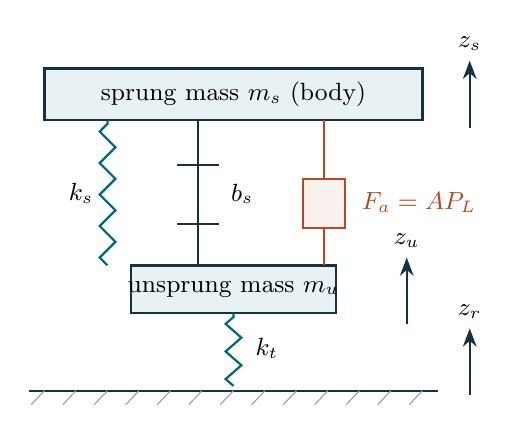
\begin{tikzpicture}[x=1cm,y=1cm,>=Stealth,thick, every node/.style={font=\small}]
  \draw[fill=accent!9,draw=ink] (1.6,3.8) rectangle (6.4,4.45);
  \node at (4,4.12) {sprung mass $m_s$ (body)};
  \draw[fill=accent!9,draw=ink] (2.7,1.35) rectangle (5.3,1.95);
  \node at (4,1.65) {unsprung mass $m_u$};
  \draw[decorate,decoration={zigzag,segment length=4mm,amplitude=1mm},draw=accent] (2.4,1.95)--(2.4,3.8);
  \node[left] at (2.35,2.87) {$k_s$};
  \draw[draw=ink] (3.55,1.95)--(3.55,2.48);
  \draw[draw=ink] (3.28,2.48)--(3.82,2.48);
  \draw[draw=ink] (3.55,2.48)--(3.55,3.23);
  \draw[draw=ink] (3.28,3.23)--(3.82,3.23);
  \draw[draw=ink] (3.55,3.23)--(3.55,3.8);
  \node[right] at (3.84,2.86) {$b_s$};
  \draw[draw=warm] (5.15,1.95)--(5.15,2.43);
  \draw[draw=warm,fill=warm!8] (4.88,2.43) rectangle (5.42,3.05);
  \draw[draw=warm] (5.15,3.05)--(5.15,3.8);
  \node[right,text=warm] at (5.5,2.75) {$F_a=A P_L$};
  \draw[decorate,decoration={zigzag,segment length=3.5mm,amplitude=1mm},draw=accent] (4,0.42)--(4,1.35);
  \node[right] at (4.15,0.9) {$k_t$};
  \draw[draw=ink] (1.4,0.36)--(6.6,0.36);
  \foreach \x in {1.6,2.0,...,6.4} {\draw[draw=muted!60,thin] (\x,0.36)--(\x-0.17,0.18);}
  \draw[->,draw=ink] (7.0,3.7)--(7.0,4.55) node[above] {$z_s$};
  \draw[->,draw=ink] (6.2,1.2)--(6.2,2.05) node[above] {$z_u$};
  \draw[->,draw=ink] (7.0,0.3)--(7.0,1.15) node[above] {$z_r$};
\end{tikzpicture}
\caption{Original vector schematic of the quarter-car model. Upward displacement is positive; the actuator force is internal to the two-mass assembly.}
\label{fig:mechanical}
\end{figure}

With suspension deflection \(d=z_s-z_u\), the model used for the numerical study is
\begin{align}
 F_s &= k_s d+k_{sn}d^3, &F_d&=b_s(\dot z_s-\dot z_u), \\
 F_t &= k_t(z_u-z_r), &F_b&=b_t(\dot z_u-\dot z_r),\\
 m_s\ddot z_s&=-F_s-F_d+F_a, &m_u\ddot z_u&=F_s+F_d-F_t-F_b-F_a.\label{eq:plant}
\end{align}
The paper's hydraulic state is \(x_5=\kappa P_L\), with \(F_a=A x_5/\kappa\), and its pressure dynamics include valve-flow and relative-velocity terms \cite{na2022}. The default simulation substitutes the \emph{equivalent} pressure-state model
\begin{equation}
 \dot x_5=-\beta x_5-c_{\rm rel}(\dot z_s-\dot z_u)+b_u u,
 \qquad |u|\leq\SI{5}{V}. \label{eq:actuator}
\end{equation}
This is not the paper's identified actuator. The nonlinear paper-valve mode exists in the code but requires rig-specific valve and fluid constants before it can be used.

\begin{table}[!htbp]
\centering\small
\caption{Numerical model values and provenance; none is presented as a measured 2022-rig constant unless marked ``paper.''}
\label{tab:provenance}
\begin{tabularx}{\linewidth}{@{}>{\raggedright\arraybackslash}p{0.24\linewidth}>{\raggedright\arraybackslash}p{0.25\linewidth}X@{}}
\toprule
Parameter & Value & Status and source\\
\midrule
\(m_s,m_u\) & 320, 40\,kg & Representative mechanical set from Jin et al. \cite{jin2019}.\\
\(k_s,k_t,b_s\) & 18, 200\,kN/m; 1\,kN\,s/m & Same separate literature set \cite{jin2019}.\\
\(k_{sn},b_t\) & 0, 0 & Simplifying assumptions.\\
\(A,\beta,P_{\max}\) & \(3.35\times10^{-4}\,\mathrm{m}^2\), \(1\,\mathrm{s}^{-1}\), 10.3425\,MPa & Illustrative actuator values motivated by a different suspension study \cite{abdulzahra2019}; not target-rig identification.\\
\(\kappa,c_{\rm rel},b_u\) & \(10^{-6}\), 0.05, 0.75 & Configurable project assumptions.\\
Sample period; command rail & 0.02\,s; \(\pm5\)\,V & From the paper's 50\,Hz implementation and valve limit \cite{na2022}.\\
\bottomrule
\end{tabularx}
\end{table}

\section{AFC with prescribed performance}
The paper applies the recursive law to \(x=[z_s,\dot z_s,z_u,\dot z_u,\kappa P_L]^\mathsf{T}\). For each channel \(i\in\{1,2,3\}\), a positive envelope
\begin{equation}
 \mu_i(t)=(\mu_{i0}-\mu_{i\infty})e^{-\alpha_i t}+\mu_{i\infty}
 \label{eq:ppf}
\end{equation}
sets the initial admissible error, convergence rate, and asymptotic tolerance. The desired constraint is \(-\delta\mu_i(t)<e_i(t)<\bar\delta\mu_i(t)\). With \(\zeta_i=e_i/\mu_i\), the inverse performance transformation is
\begin{equation}
 \epsilon_i=\frac12\ln\left(\frac{\delta+\zeta_i}{\bar\delta-\zeta_i}\right),
 \qquad -\delta<\zeta_i<\bar\delta.
 \label{eq:transform}
\end{equation}
The recursive AFC equations are
\begin{align}
 e_1&=x_1, &u_1&=-k_1\epsilon_1,\\
 e_2&=x_2-u_1, &u_2&=-k_2\epsilon_2,\\
 e_3&=x_5-u_2, &u&=-k_3\epsilon_3. \label{eq:afc}
\end{align}
Unlike model-based backstepping, the proportional-like transformed-error recursion does not explicitly differentiate its virtual controls or employ a neural/fuzzy function approximator \cite{na2022}. This does not make actuator authority unlimited: clipping \(u\) may invalidate the assumptions behind the unsaturated envelope guarantee.
The code also applies a small open-interval guard to \(\zeta_i\) before evaluating the logarithm; this prevents a numerical singularity but does not restore PPF compliance once the physical trajectory has crossed a bound.

\begin{table}[!htbp]
\centering\small
\caption{Paper Case A tuning used in the simulation. The symmetric \(\delta=\bar\delta=1\) choice is a project inference from the plotted bounds, not a tabulated paper value.}
\label{tab:caseA}
\begin{tabular}{@{}lrrrr@{}}
\toprule
Channel & \(\mu_{i0}\) & \(\mu_{i\infty}\) & \(\alpha_i\) & \(k_i\)\\
\midrule
Body displacement, \(i=1\) & 0.2 & 0.018 & 3 & 25.5\\
Virtual velocity error, \(i=2\) & 110 & 90 & 2 & 12\\
Scaled-pressure error, \(i=3\) & 100 & 80 & 2 & 216\\
\bottomrule
\end{tabular}
\end{table}

\section{Reproduction protocol and implementation}
The MATLAB script samples each controller at 50\,Hz and integrates the five-state plant with four RK4 substeps per sample. The Simulink implementation uses an editable MATLAB Function AFC block, a zero-order hold, a plant block, and a fixed-step \texttt{ode4} solver. Figure~\ref{fig:simulink} is an actual programmatic export of the working \texttt{.slx} diagram, not a recreated drawing. The model logs road, body states, command, and acceleration. The MATLAB comparison adds BSC, PID, and passive runs; it uses full simulated state feedback and does not reproduce the experimental observer or sensor chain.

\begin{figure}[!htbp]
\centering
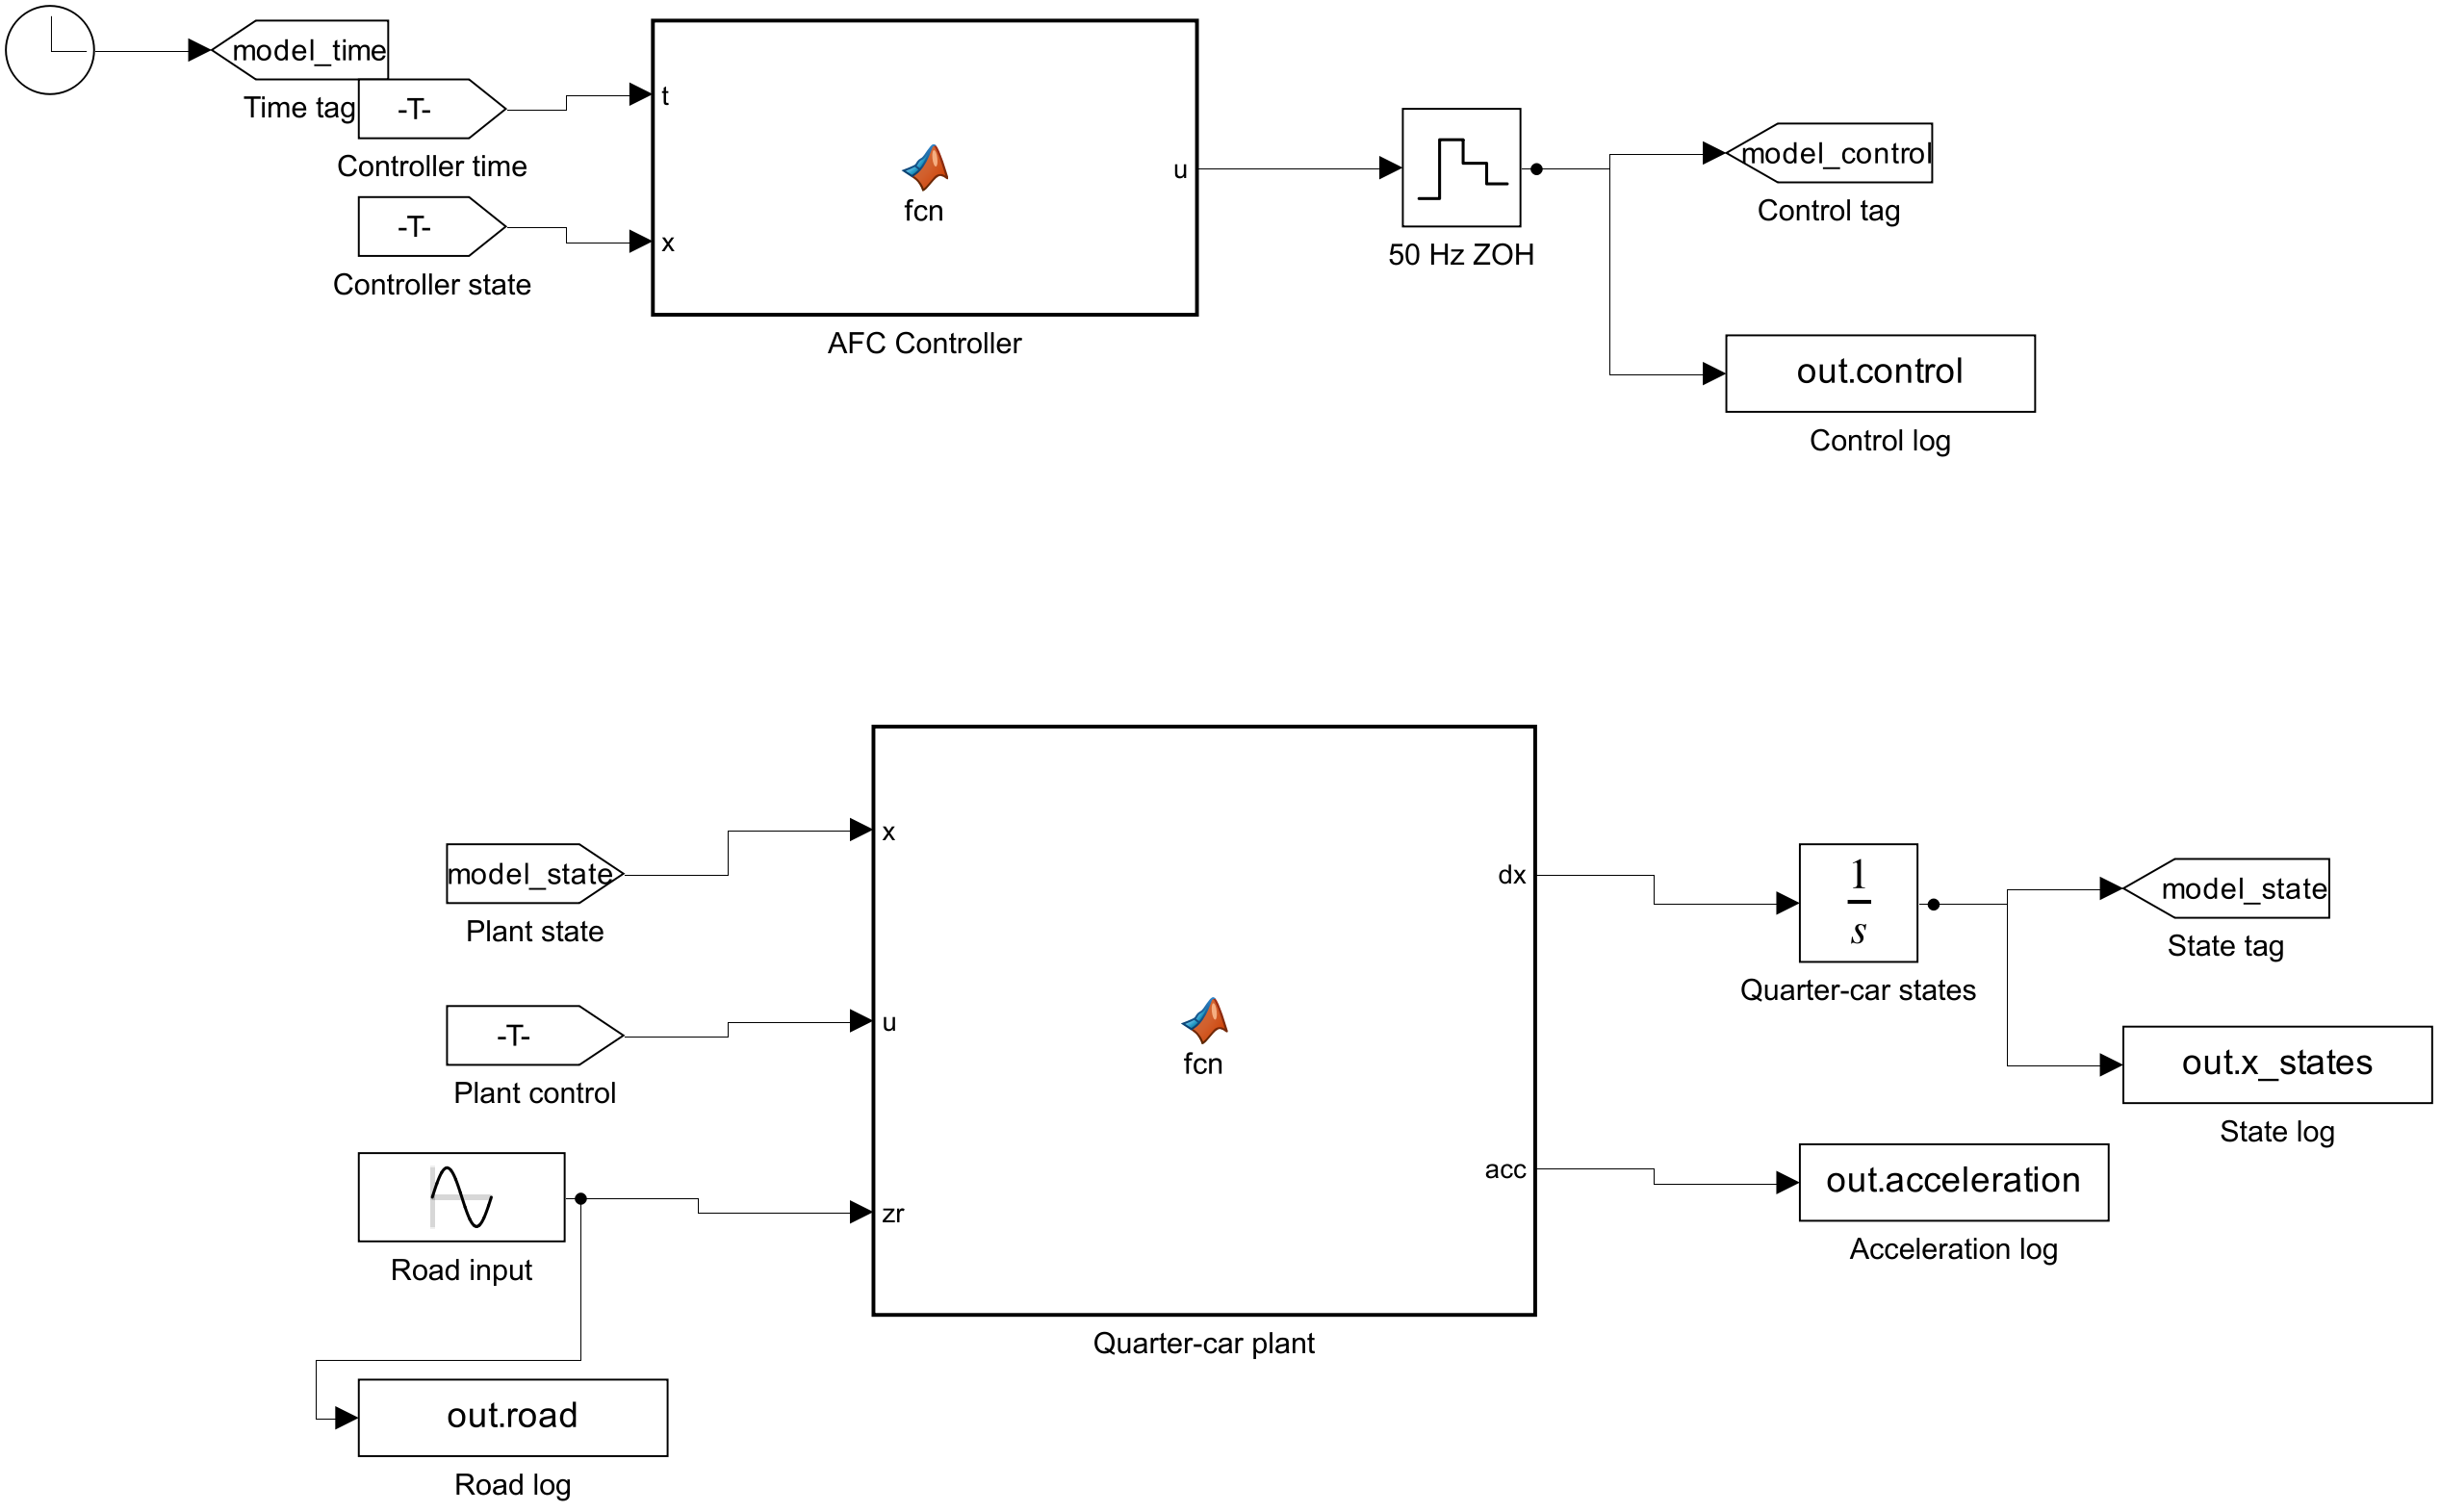
\includegraphics[width=0.96\linewidth]{paper_assets/simulink_model.png}
\caption{Actual executable Simulink model: AFC, 50\,Hz hold, road input, plant, state integration, and logs. Tagged connections avoid long feedback wires.}
\label{fig:simulink}
\end{figure}

For the principal comparison, the road is \(z_r(t)=0.043\sin(2\pi\,0.505t)\,\mathrm{m}\) over 20\,s (the paper's 10-peak sinusoidal case). The eight-case sweep uses the paper's amplitude/frequency pairs: \((0.025,0.188)\), then \((0.043,0.204)\), \((0.043,0.243)\), \((0.043,0.307)\), \((0.043,0.361)\), \((0.043,0.407)\), \((0.043,0.423)\), and \((0.043,0.505)\), in metres and hertz \cite{na2022}. This project's sweep holds the Case A AFC gains fixed, whereas the paper retunes several slower cases.

For a displacement trace \(z_s(t)\) and horizon \(T\), the computed indices are
\begin{equation}
 \mathrm{IAE}=\int_0^T |z_s|\,dt,\quad
 \mathrm{ITAE}=\int_0^T t|z_s|\,dt,\quad
 \mathrm{ITSE}=\int_0^T t z_s^2\,dt.
 \label{eq:indices}
\end{equation}
Acceleration RMS, command RMS, saturation fraction, and maximal positive violation of \(\pm\mu_1\) are evaluated on the sampled trajectory. Separate code paths for numerical integration and Simulink permit an implementation cross-check.

\section{Results: representative simulation}
\subsection{Road response and prescribed-envelope audit}
Figure~\ref{fig:response} presents the actual MATLAB traces for the 10-peak road input. All active controllers improve IAE relative to passive operation, but the present assumed plant does not recover the paper's experimental ranking: PID has slightly lower IAE than AFC. Figure~\ref{fig:ppf} keeps the full initial \(\pm0.2\,\mathrm{m}\) envelope visible and adds the normalized ratio \(|z_s|/\mu_1\); values above one mark violations unambiguously. The worst violation is \SI{0.01885}{m}.

\begin{figure}[!htbp]
\centering
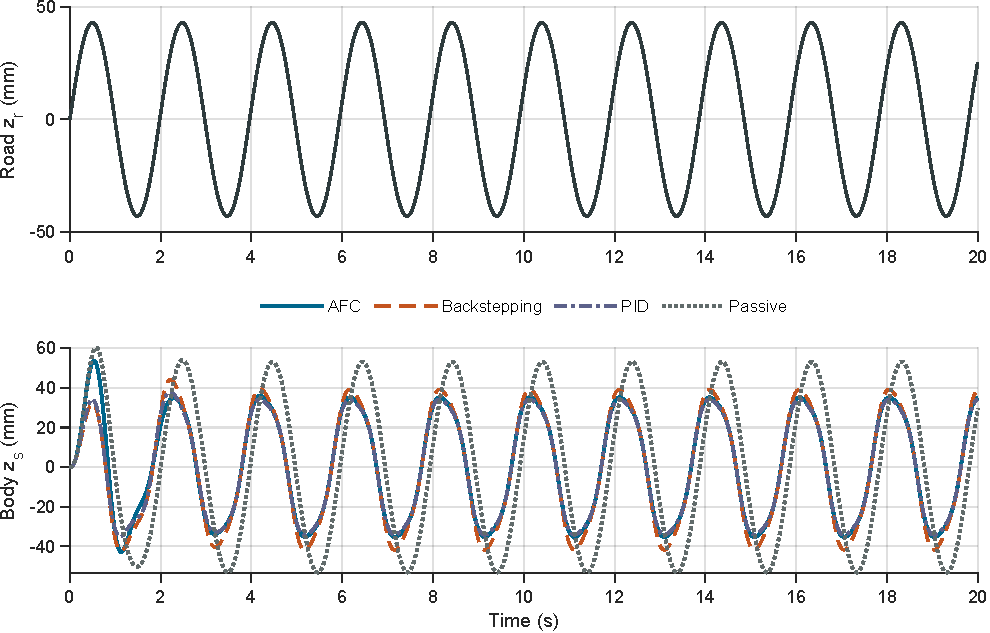
\includegraphics[width=0.95\linewidth]{paper_assets/response_comparison.pdf}
\caption{\textsc{Simulation}: 10-peak sinusoidal road and body displacement. All plotted trajectories come from \texttt{quarter\_car\_replication\_results.mat}.}
\label{fig:response}
\end{figure}

\begin{figure}[!htbp]
\centering
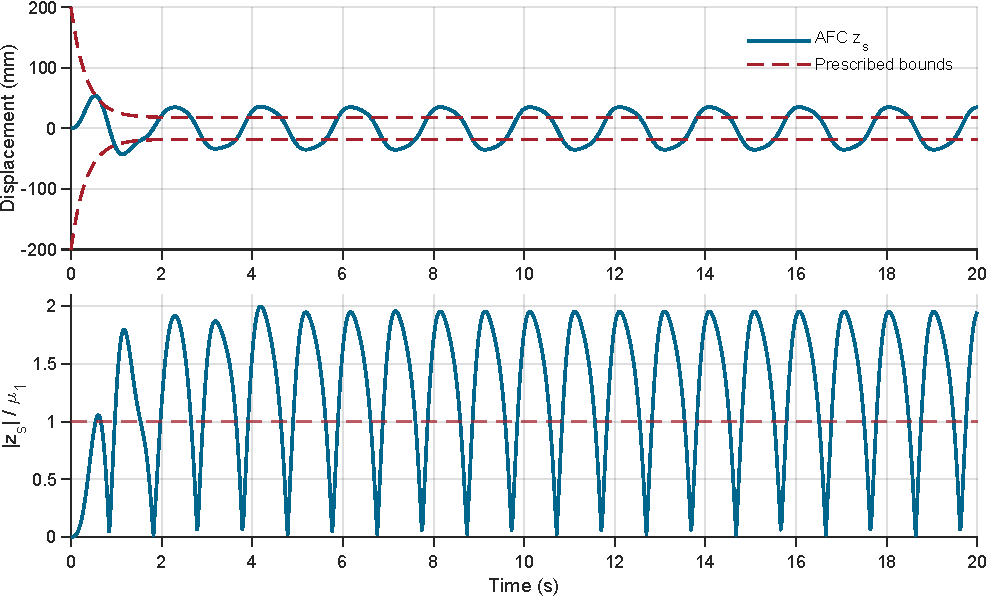
\includegraphics[width=0.95\linewidth]{paper_assets/ppf_audit.pdf}
\caption{\textsc{Simulation}: AFC body displacement against the assumed symmetric Case A envelope. The lower ratio panel shows where the prescribed bound is exceeded.}
\label{fig:ppf}
\end{figure}
\FloatBarrier

\subsection{Acceleration, voltage, and aggregate error}
Figure~\ref{fig:actuation} shows the simulated body acceleration and saturated AFC command. The raw command exceeds the \(\pm\SI{5}{V}\) limit on 85.4\% of samples, so applying the unconstrained recursive law is not what the simulated plant experiences. The sampled acceleration RMS values are about 0.3894\,m/s\(^2\) for AFC and 0.3965\,m/s\(^2\) for passive. These are not directly comparable to the paper's fixed-waveform hardware RMS because both the excitation and the physical rig differ.

\begin{figure}[!htbp]
\centering
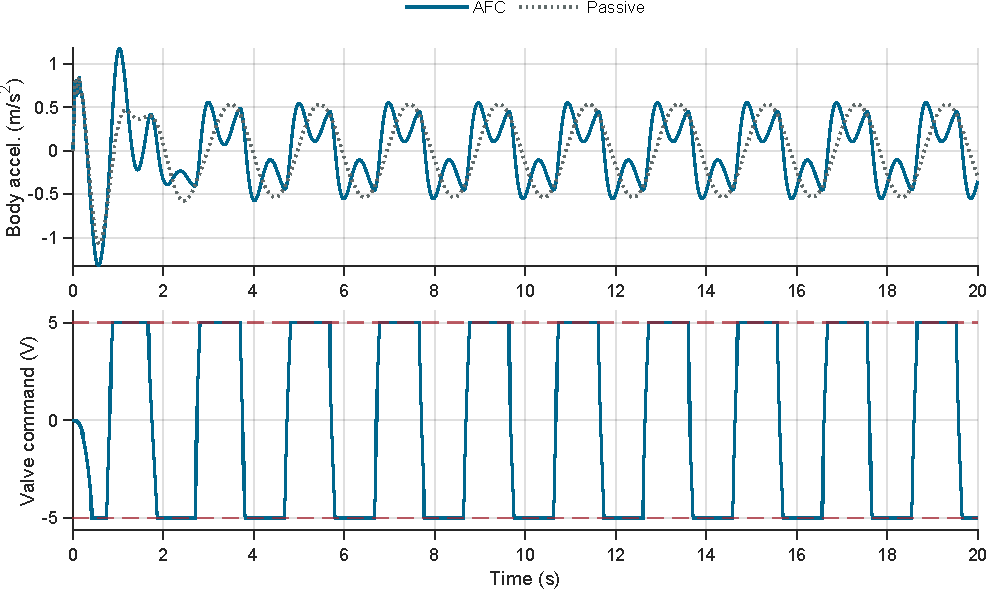
\includegraphics[width=0.95\linewidth]{paper_assets/acceleration_control.pdf}
\caption{\textsc{Simulation}: body acceleration and applied AFC valve voltage. Dashed horizontal lines show the \(\pm\SI{5}{V}\) rails.}
\label{fig:actuation}
\end{figure}

\begin{table}[!htbp]
\centering\small
\caption{\textsc{Simulation}: Case 10 aggregate measures over 20\,s. Lower is preferable within each metric; no entry is a measurement from the paper.}
\label{tab:metrics}
\begin{tabular}{@{}lrrrr@{}}
\toprule
Controller & IAE (m\,s) & ITAE (m\,s\(^2\)) & ITSE (m\(^2\)\,s\(^2\)) & Acc. RMS (m/s\(^2\))\\
\midrule
AFC & 0.4849 & 4.8070 & 0.1369 & 0.3894\\
BSC & 0.5248 & 5.2841 & 0.1686 & 0.3921\\
PID & \textbf{0.4698} & \textbf{4.7166} & \textbf{0.1309} & \textbf{0.3676}\\
Passive & 0.6709 & 6.6983 & 0.2784 & 0.3965\\
\bottomrule
\end{tabular}
\end{table}

\begin{figure}[!htbp]
\centering
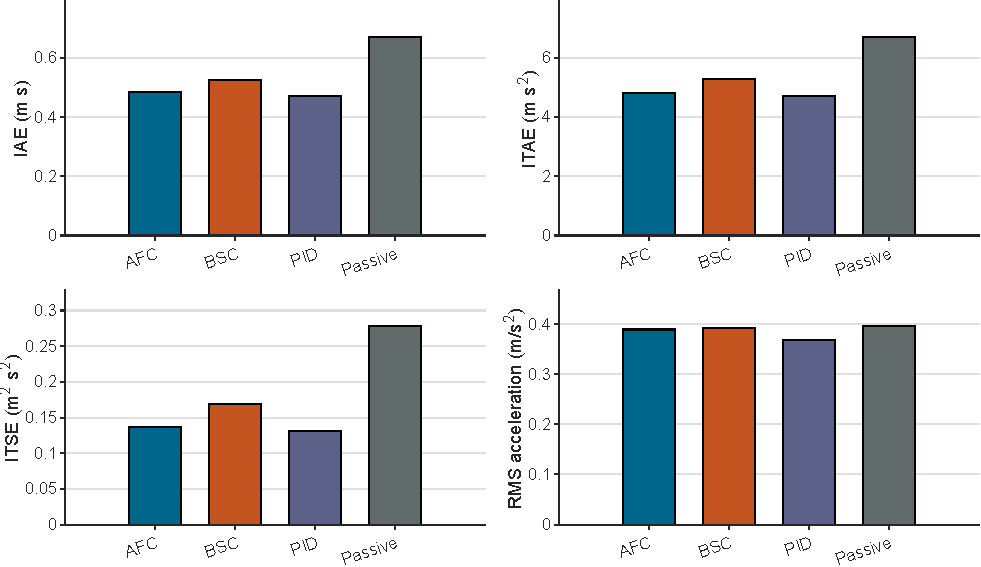
\includegraphics[width=0.93\linewidth]{paper_assets/metric_comparison.pdf}
\caption{\textsc{Simulation}: the four controller comparisons in Table~\ref{tab:metrics}; axes retain their physical units.}
\label{fig:metrics}
\end{figure}
\FloatBarrier

\subsection{Road-condition sweep and independent solver check}
Figure~\ref{fig:sweep} gives IAE, ITAE, and ITSE for the eight AFC road inputs with fixed Case A tuning. The indices are not monotonic in peak count because frequency, amplitude, finite simulation duration, and fixed gains all change the response. This is a model sensitivity study, not a digitization of the paper's road-sweep data. Figure~\ref{fig:crosscheck} overlays the MATLAB RK4 and Simulink \texttt{ode4} AFC trajectories. Agreement checks that the two code paths implement the same chosen model; it does not identify the true rig.

\begin{figure}[!htbp]
\centering
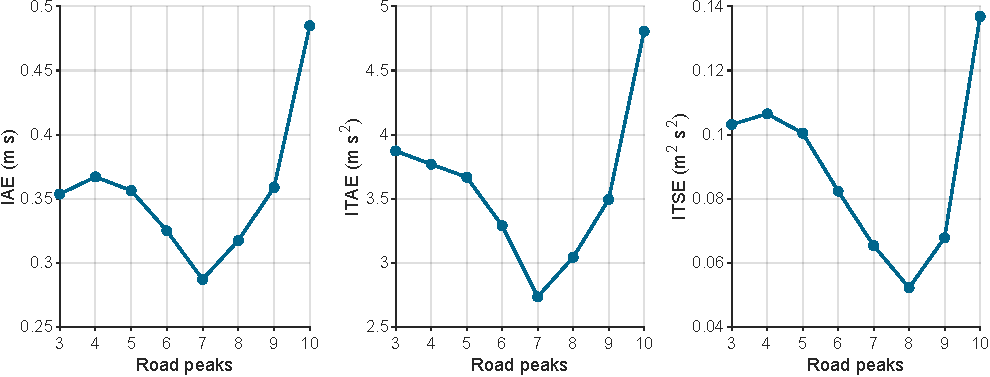
\includegraphics[width=0.98\linewidth]{paper_assets/road_sweep.pdf}
\caption{\textsc{Simulation}: AFC indices for the paper's eight sinusoidal input pairs, with one fixed controller tuning.}
\label{fig:sweep}
\end{figure}

\begin{figure}[!htbp]
\centering
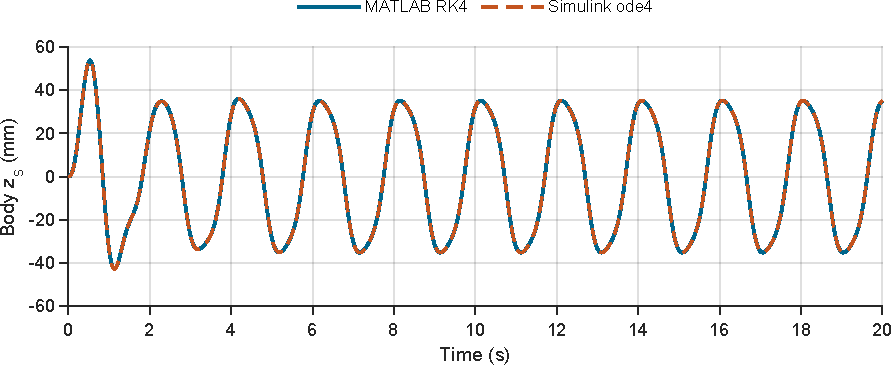
\includegraphics[width=0.9\linewidth]{paper_assets/implementation_crosscheck.pdf}
\caption{\textsc{Simulation}: independently executed MATLAB and Simulink AFC trajectories for the 10-peak input. Solver steps differ (MATLAB 0.005\,s RK4 substep; Simulink 0.001\,s fixed-step \texttt{ode4}).}
\label{fig:crosscheck}
\end{figure}
\FloatBarrier

\section{Interpretation and reproducibility boundary}
The source paper reports PPF-compliant experimental displacement and superior AFC error indices for its rig \cite{na2022}. Our representative-model run instead exposes a feasibility failure: the modeled actuator is commonly at its voltage rail, the body trajectory leaves the prescribed envelope, and PID narrowly leads the chosen metrics. This disagreement cannot be attributed to one cause without identification data. It may reflect the surrogate pressure dynamics, target-rig parameter differences, selected gains, nonlinear valve effects, or the missing sensor/observer path. The PPF guarantee for an ideal unsaturated law should not be silently extended to clipped control.

The project is reproducible by running the supplied MATLAB replication and figure-generation scripts in order (MATLAB R2024b with Simulink). The configuration file exposes all assumed constants. To pursue a quantitative replication, obtain or identify the hydraulic valve and rig constants; acquire the original road and measured signals; implement the paper's force observer and sensor processing; reproduce its case-specific retuning; then compare aligned displacement, acceleration, valve voltage, and envelope-violation metrics. The publisher PDF is intentionally not redistributed in the public project repository.

\section{Conclusion}
AFC with PPFs makes transient constraints explicit and retains a compact recursive implementation. A runnable MATLAB/Simulink reproduction confirms the equations can be exercised and plotted, but the representative actuator does not sustain the paper's claimed envelope for the demanding sinusoidal case. The scientifically defensible result is therefore a well-instrumented partial reproduction with a clearly identified hardware-data gap, not a claimed experimental validation.

\small
\begin{thebibliography}{9}
\bibitem{na2022} J. Na, Y. Huang, X. Wu, Y.-J. Liu, Y. Li, and G. Li, ``Active Suspension Control of Quarter-Car System With Experimental Validation,'' \emph{IEEE Transactions on Systems, Man, and Cybernetics: Systems}, vol. 52, no. 8, pp. 4714--4726, 2022. \href{https://doi.org/10.1109/TSMC.2021.3103807}{doi:10.1109/TSMC.2021.3103807}.
\bibitem{jin2019} P. Jin, W. Xue, and K. Li, ``Actuator Fault Estimation for Vehicle Active Suspensions Based on Adaptive Observer and Genetic Algorithm,'' \emph{Shock and Vibration}, 2019, Article ID 1783850. \href{https://doi.org/10.1155/2019/1783850}{doi:10.1155/2019/1783850}.
\bibitem{abdulzahra2019} A. K. Abdulzahra and T. Y. Abdalla, ``Fuzzy Sliding Mode Control Scheme for Vehicle Active Suspension System Optimized by ABC Algorithm,'' \emph{International Journal of Intelligent Systems and Applications}, vol. 11, no. 12, pp. 1--10, 2019. \href{https://doi.org/10.5815/ijisa.2019.12.01}{doi:10.5815/ijisa.2019.12.01}.
\end{thebibliography}
\end{document}
